\section{Referenciação entre labels em \LaTeX}
\begin{frame}[fragile]
\begin{block}{}
\begin{itemize}
 \item Em \LaTeX você pode facilmente referenciar quase tudo que é enumerado (sections, figures, formulas), e o \LaTeX irá  tratar o que for necessário para essas referências, atualizando sempe que houver modificações.
\end{itemize}
\end{block}
\end{frame}

\begin{frame}[fragile]
\begin{description}[maiortextodomundoqueconsigoes]
		\item [{\code \textbackslash label\{marker\}}]	Marca um objeto para futura referência
		\item [{\code \textbackslash ref\{marker\}}]    Referencia um objeto marcado
		\item [{\code \textbackslash pageref\{marker\}}]    Imprime o numero da página do objeto marcado
		\item [{\code \textbackslash nameref\{marker\}}]    Imprime o que estiver no caption do objeto marcado
	\end{description}
\end{frame}

\subsection*{Exemplo de referência de uma section}

\begin{frame}[fragile]

Exemplo de referência de uma section:

\lstinputlisting[linewidth=10cm]{citacoes/sectionExamples.tex}

\end{frame}

\begin{frame}[fragile]

Output do código anterior:

\begin{figure}[p]
   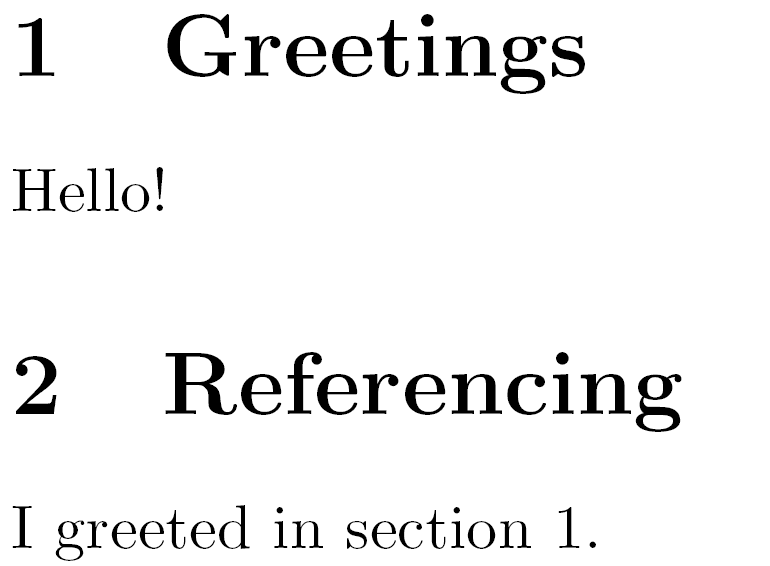
\includegraphics[scale=0.5]{figuras/sectionExample.png}
\end{figure}

\end{frame}